\documentclass[a4paper,12pt]{article} % тип документа

% report, book

% Рисунки
\usepackage{graphicx}
\usepackage{wrapfig}
\usepackage{mathtext}
\usepackage[left=2cm,right=2cm,
    top=2cm,bottom=2cm,bindingoffset=0cm]{geometry}

\usepackage{hyperref}
\usepackage[rgb]{xcolor}
\hypersetup{				% Гиперссылки
    colorlinks=true,       	% false: ссылки в рамках
	urlcolor=blue          % на URL
}

%  Русский язык
\usepackage[T2A]{fontenc}			% кодировка
\usepackage[utf8]{inputenc}			% кодировка исходного текста
\usepackage[english,russian]{babel}	% локализация и переносы
\addto\captionsrussian{\def\refname{Список используемой литературы}}


% Математика
\usepackage{amsmath,amsfonts,amssymb,amsthm,mathtools} 
\usepackage{titlesec}
\titlelabel{\thetitle.\quad}

\usepackage{wasysym}

\begin{document}\begin{titlepage}

\thispagestyle{empty}

\centerline{МОСКОВСКИЙ ФИЗИКО-ТЕХНИЧЕСКИЙ ИНСТИТУТ}
\centerline{(НАЦИОНАЛЬНЫЙ ИССЛЕДОВАТЕЛЬСКИЙ УНИВЕРСИТЕТ)}

\vfill

\centerline{\huge{Лабораторная работа 3.6.1}}
\centerline{\large{по теме:}}
\centerline{\LARGE{<<Спектральный анализ электрических сигналов>>}}

\vfill

Студент группы Б02-109 \hfill Назарчук Анна

\vfill

\centerline{Долгопрудный, 2022}
\clearpage
\end{titlepage} 
\section{Аннотация}
В работе исследованы спектры периодических сигналов: модулированный по амплитуде, прямоугольные импульсы и цуги. Проверены теоретические зависимости параметров спектра на практике.


\section{Введение}
Многие практические задачи описания поведения некоторой системы во времени зачастую сводятся к выяснению связи между "сигналом", подаваемым на "вход"
системы (обозначим его как $f(t)$), и её реакцией на "выходе" $g(t)$). Суть спектрального метода состоит в представлении произвольного воздействия в виде суперпозиции откликов на некоторые элементарные слагаемые. Данный метод используются для анализа многих сигналов, поэтому необходимо экспериментально ознакомиться с ним, сгенерировать и получить на осциллографе спектры различных периодических сигналов, проверить экспериментально соотношение неопределенности и отношения амплитуд гармоник при модулированных по амплитуде сигналах.

\section{Методика измерений}
Для экспериментальной проверки соотношения неопределенностей необходимо его сформулировать \cite{labnik}:
\begin{equation}
\Delta \omega \cdot \Delta t \sim 2\pi
\end{equation}
Для проверки соотношения неопределенностей работа разделена на три равноценные части, в каждой из которых сгенерирован сигнал определенной формы, обработан с помощью цифрового осциллографа, проверены соотношения неопределенности с помощью курсорных измерений.
1. Первая часть работы заключалась в исследовании спектра периодической последовательности прямоугольных импульсов (пример показан на рисунке \ref{прямоуг}). 
\begin{figure}[h!]
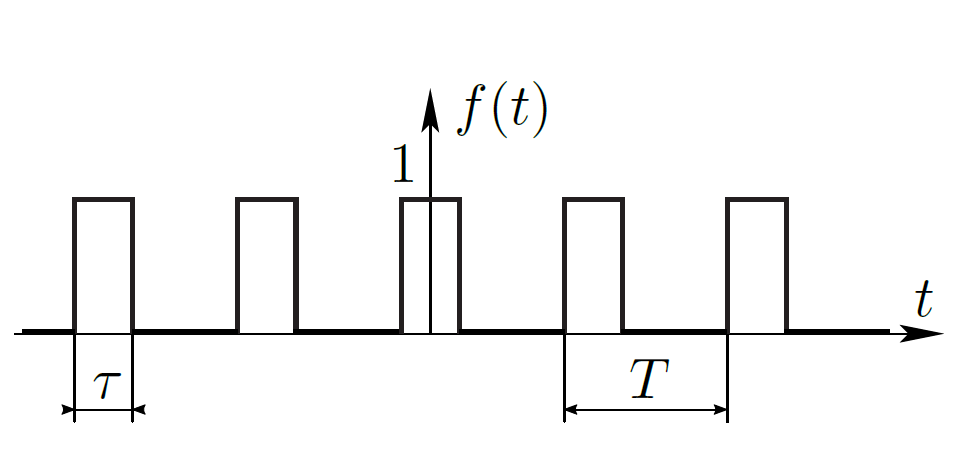
\includegraphics[width=0.4\textwidth]{rect}
\caption{Пример периодической последовательности прямоугольных импульсов из \cite{labnik}} \label{rect}
\end{figure}
Теоретически рассчитано значение коэффициентов $c_n$ \cite{labnik}:
\begin{equation}
c_n  = \dfrac{sin(\pi n \tau / T))}{\pi n}
\end{equation}

2. Вторая часть работы состояла в исследовании спектра периодической последовательности цугов гармонических колебаний (пример показан на рисунке \ref{цуги}). 
\begin{figure}[h!]
\begin{center}
\includegraphics[width=0.4\textwidth]{цуги}
\caption{Пример периодической последовательности цуг из \cite{labnik}} \label{цуги}
\end{center}
\end{figure}
Теоретически известен спектр сигнала \cite{labnik}: 
\begin{equation}
F(\omega) = \dfrac{\tau}{2T}\left[\dfrac{\sin(\omega-\omega_0)\tau /2}
{(\omega-\omega_0)\tau /2}
 + \dfrac{\sin(\omega+\omega_0)\tau /2}{(\omega+\omega_0)\tau /2}\right]
\end{equation}

3. Последняя часть заключалась в исследовании спектра гармонических сигналов, модулированных по амплитуде  (пример показан на рисунке \ref{модулированный}).
\begin{figure}[h!]
\begin{center}
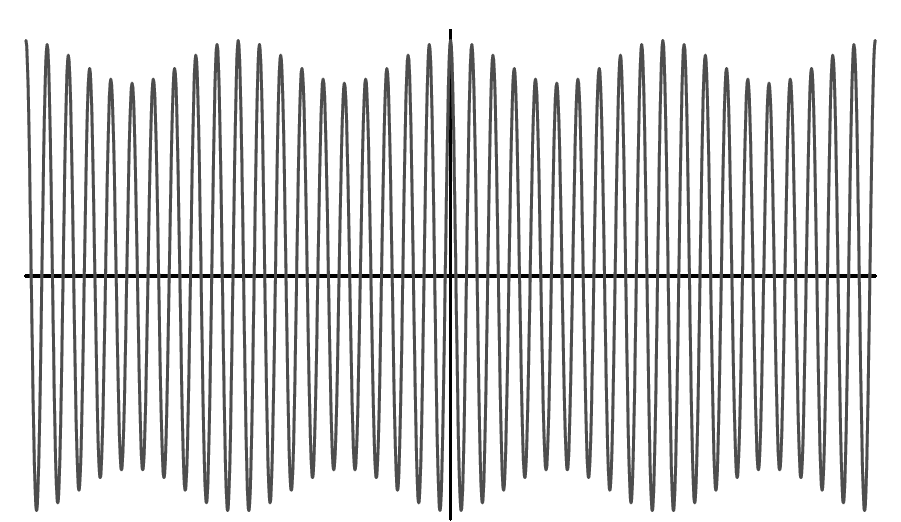
\includegraphics[width=0.4\textwidth]{Модулированный}
\caption{Пример модулированного по амплитуде сигнала из \cite{labnik}} \label{модулированный}
\end{center}
\end{figure}
Теоретический вид сигнала \cite{labnik}: 
\begin{equation}
f(t) = a_0 \cos (\omega_0 t) +\dfrac{ma_0}{2}\cos (\omega_0 +\Omega)t++\dfrac{ma_0}{2}\cos (\omega_0 -\Omega)t
\end{equation}



\section{Измерения и обработка данных}
\subsection*{Исследования спектра периодической последовательности прямоугольных импульсов}
Для исследования периодической последовательности прямоугольных импульсов на генераторе создан сигнал с разными параметрами, по которому на экране осциллографа получается спектр (рис. \ref{прямоуг})

\begin{figure}[h!]
\begin{minipage}[h!]{0.47\linewidth}
\center{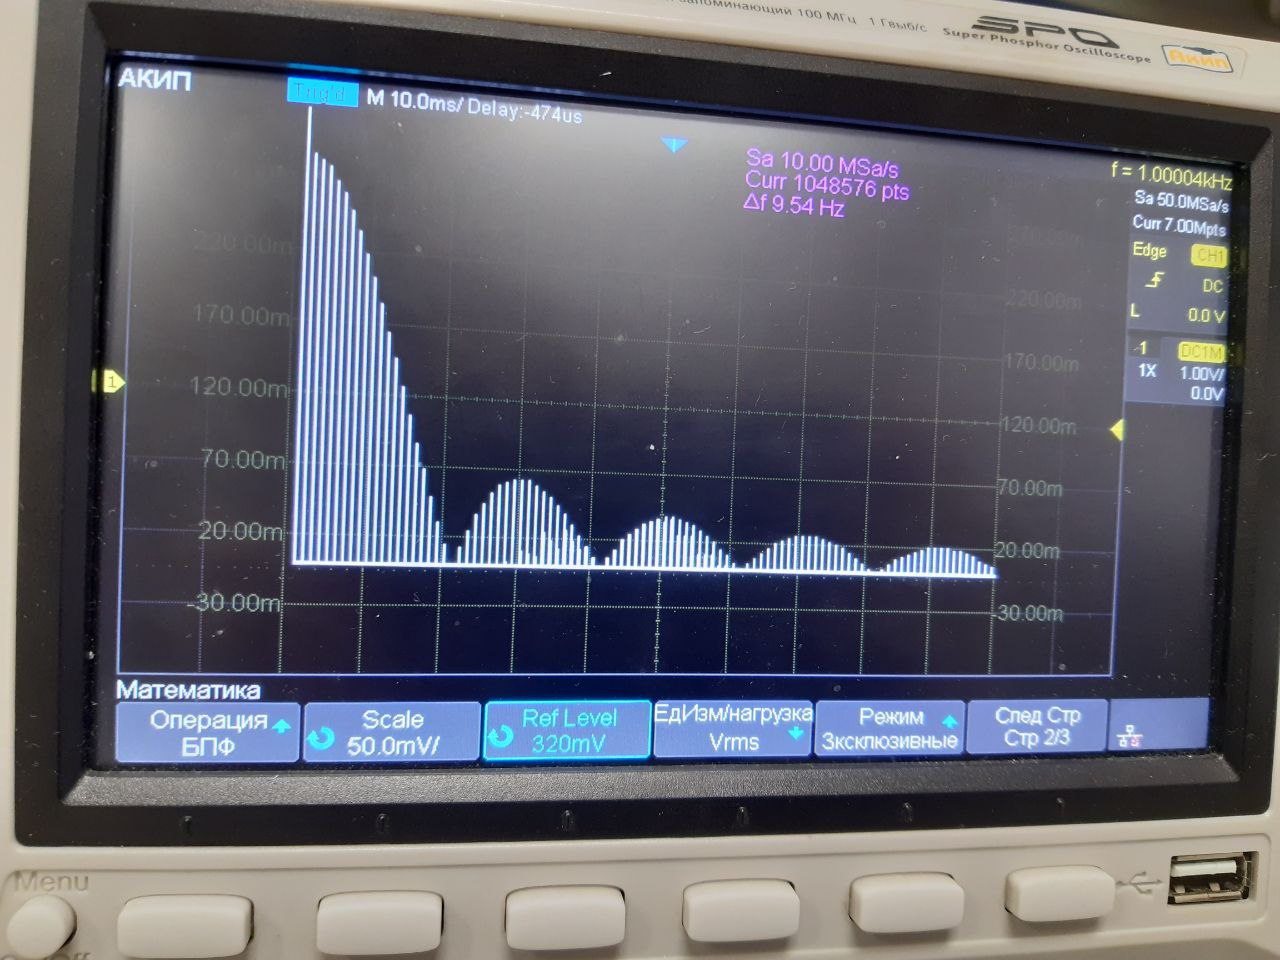
\includegraphics[width=1\linewidth]{1_1}} a) $\nu_{повт} = 1000 Гц, \tau = 50 мкс$\\
\end{minipage}
\hfill
\begin{minipage}[h!]{0.47\linewidth}
\center{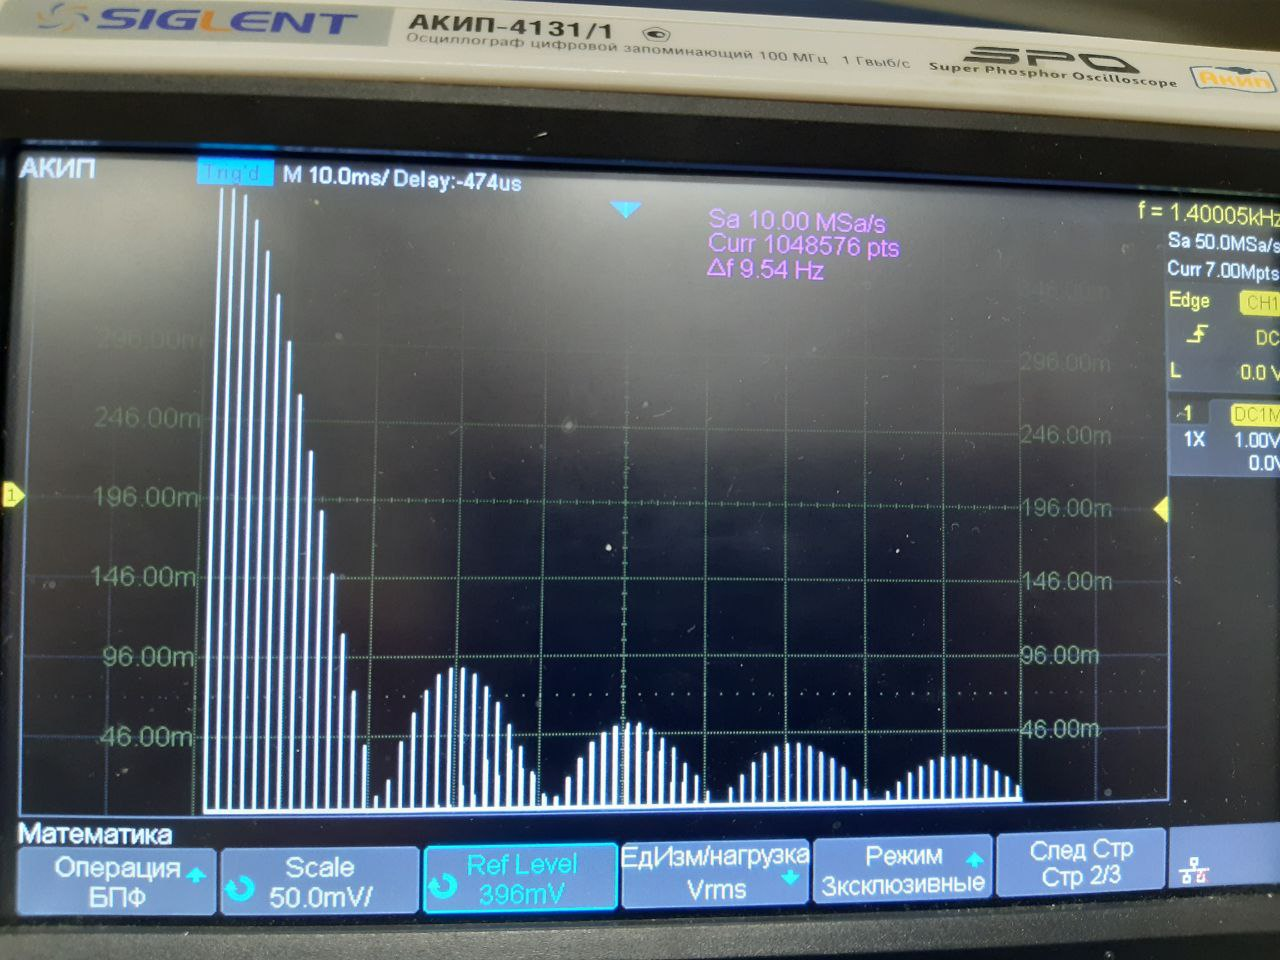
\includegraphics[width=1\linewidth]{1_2}} \\b) $\nu_{повт} = 1400 Гц, \tau = 50 мкс$
\end{minipage}
\vfill
\begin{minipage}[h!]{0.47\linewidth}
\center{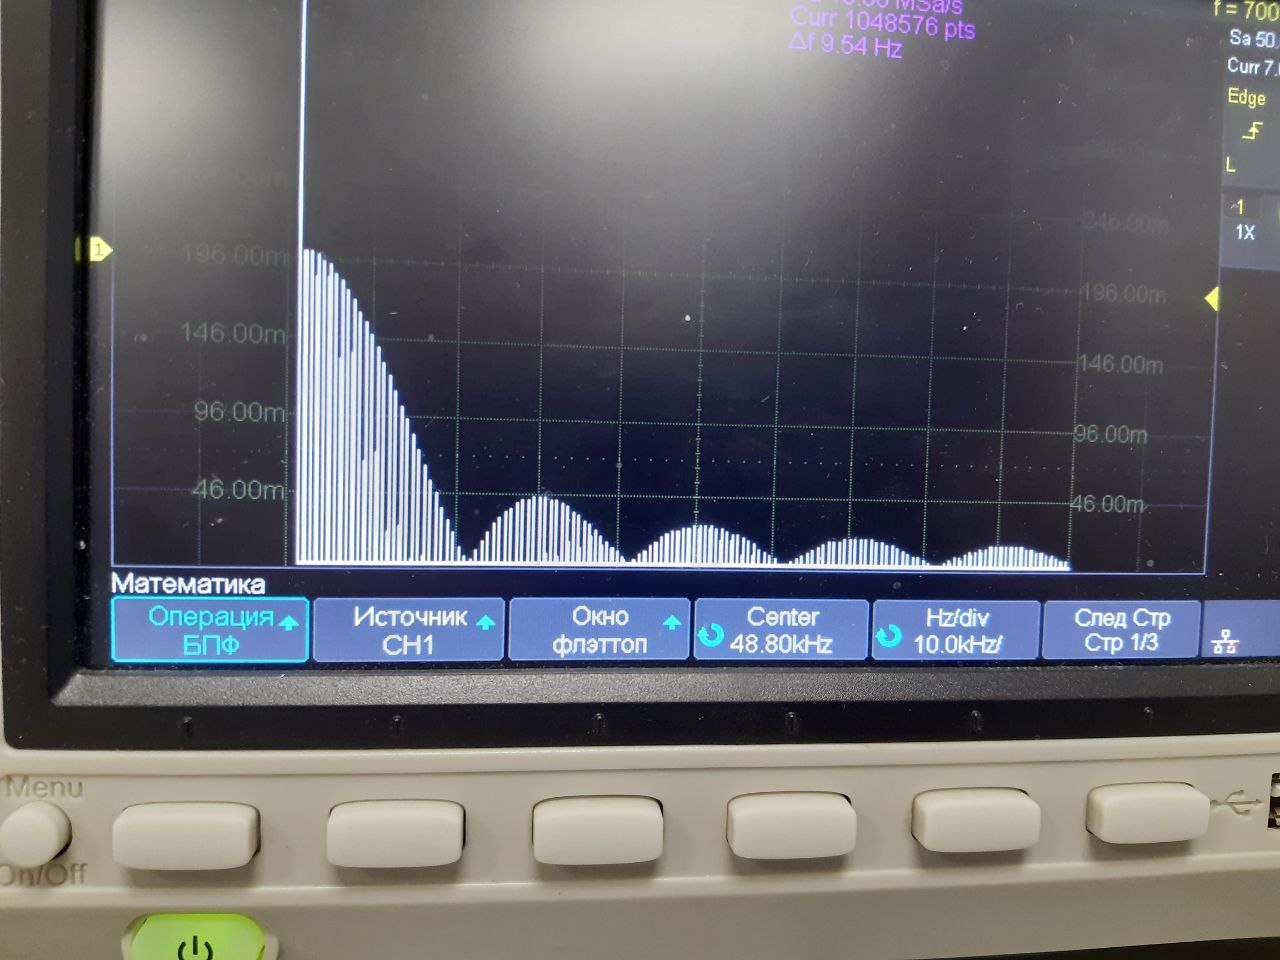
\includegraphics[width=1\linewidth]{1_3}} c) $\nu_{повт} = 700 Гц, \tau = 50 мкс$ \\
\end{minipage}
\hfill
\begin{minipage}[h!]{0.47\linewidth}
\center{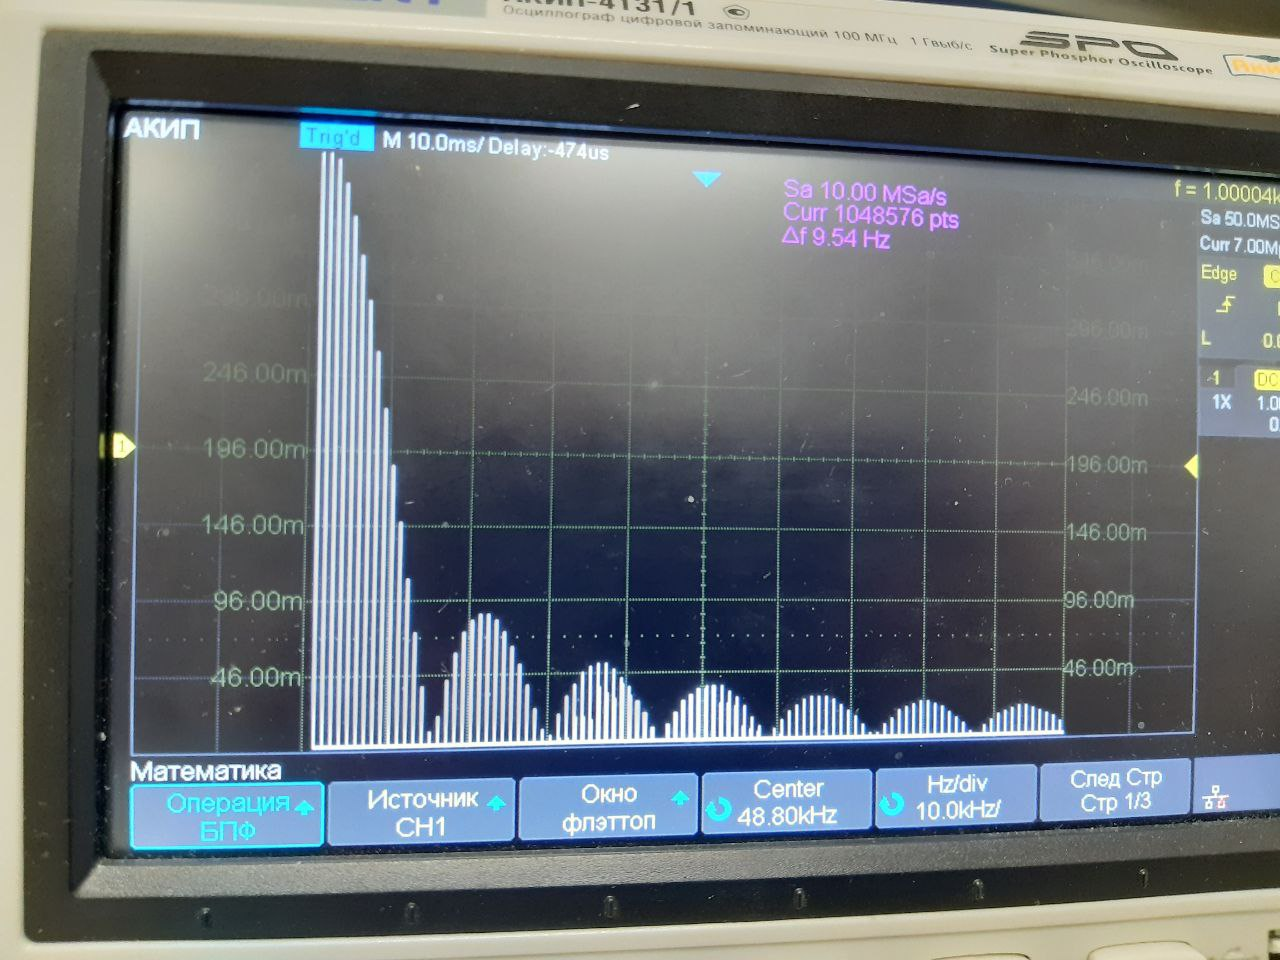
\includegraphics[width=1\linewidth]{1_4}} d) $\nu_{повт} = 1000 Гц, \tau = 70 мкс$ \\
\end{minipage}
\caption{Спектры последовательностей прямоугольных импульсов при разных частотах повторения и длительности импульса}
\label{прямоуг}
\end{figure}
При $\nu_{повт} = 700 Гц$ проведены измерения ширины спектра. Результаты 
представлены в таблице \ref{dnu(tau)_tbl} и на рисунке \ref{dnu(tau)_img}.
\begin{table}[h!]
\caption{Зависимость ширины спектра от длительности спектра для последовательности прямоугольных импульсов при $\nu_{повт} = 700 Гц$} \label{dnu(tau)_tbl}
\begin{tabular}{|l|l|}
\hline
$\Delta\nu$, Hz & $\tau$, мкс \\ \hline
50200         & 20       \\ \hline
25200         & 40       \\ \hline
17200         & 60       \\ \hline
13000         & 80       \\ \hline
10200         & 100      \\ \hline
8600          & 120      \\ \hline
7400          & 140      \\ \hline
6600          & 160      \\ \hline
5800          & 180      \\ \hline
5000          & 200      \\ \hline
\end{tabular}
\end{table}

\begin{figure}[h!]
\begin{center}
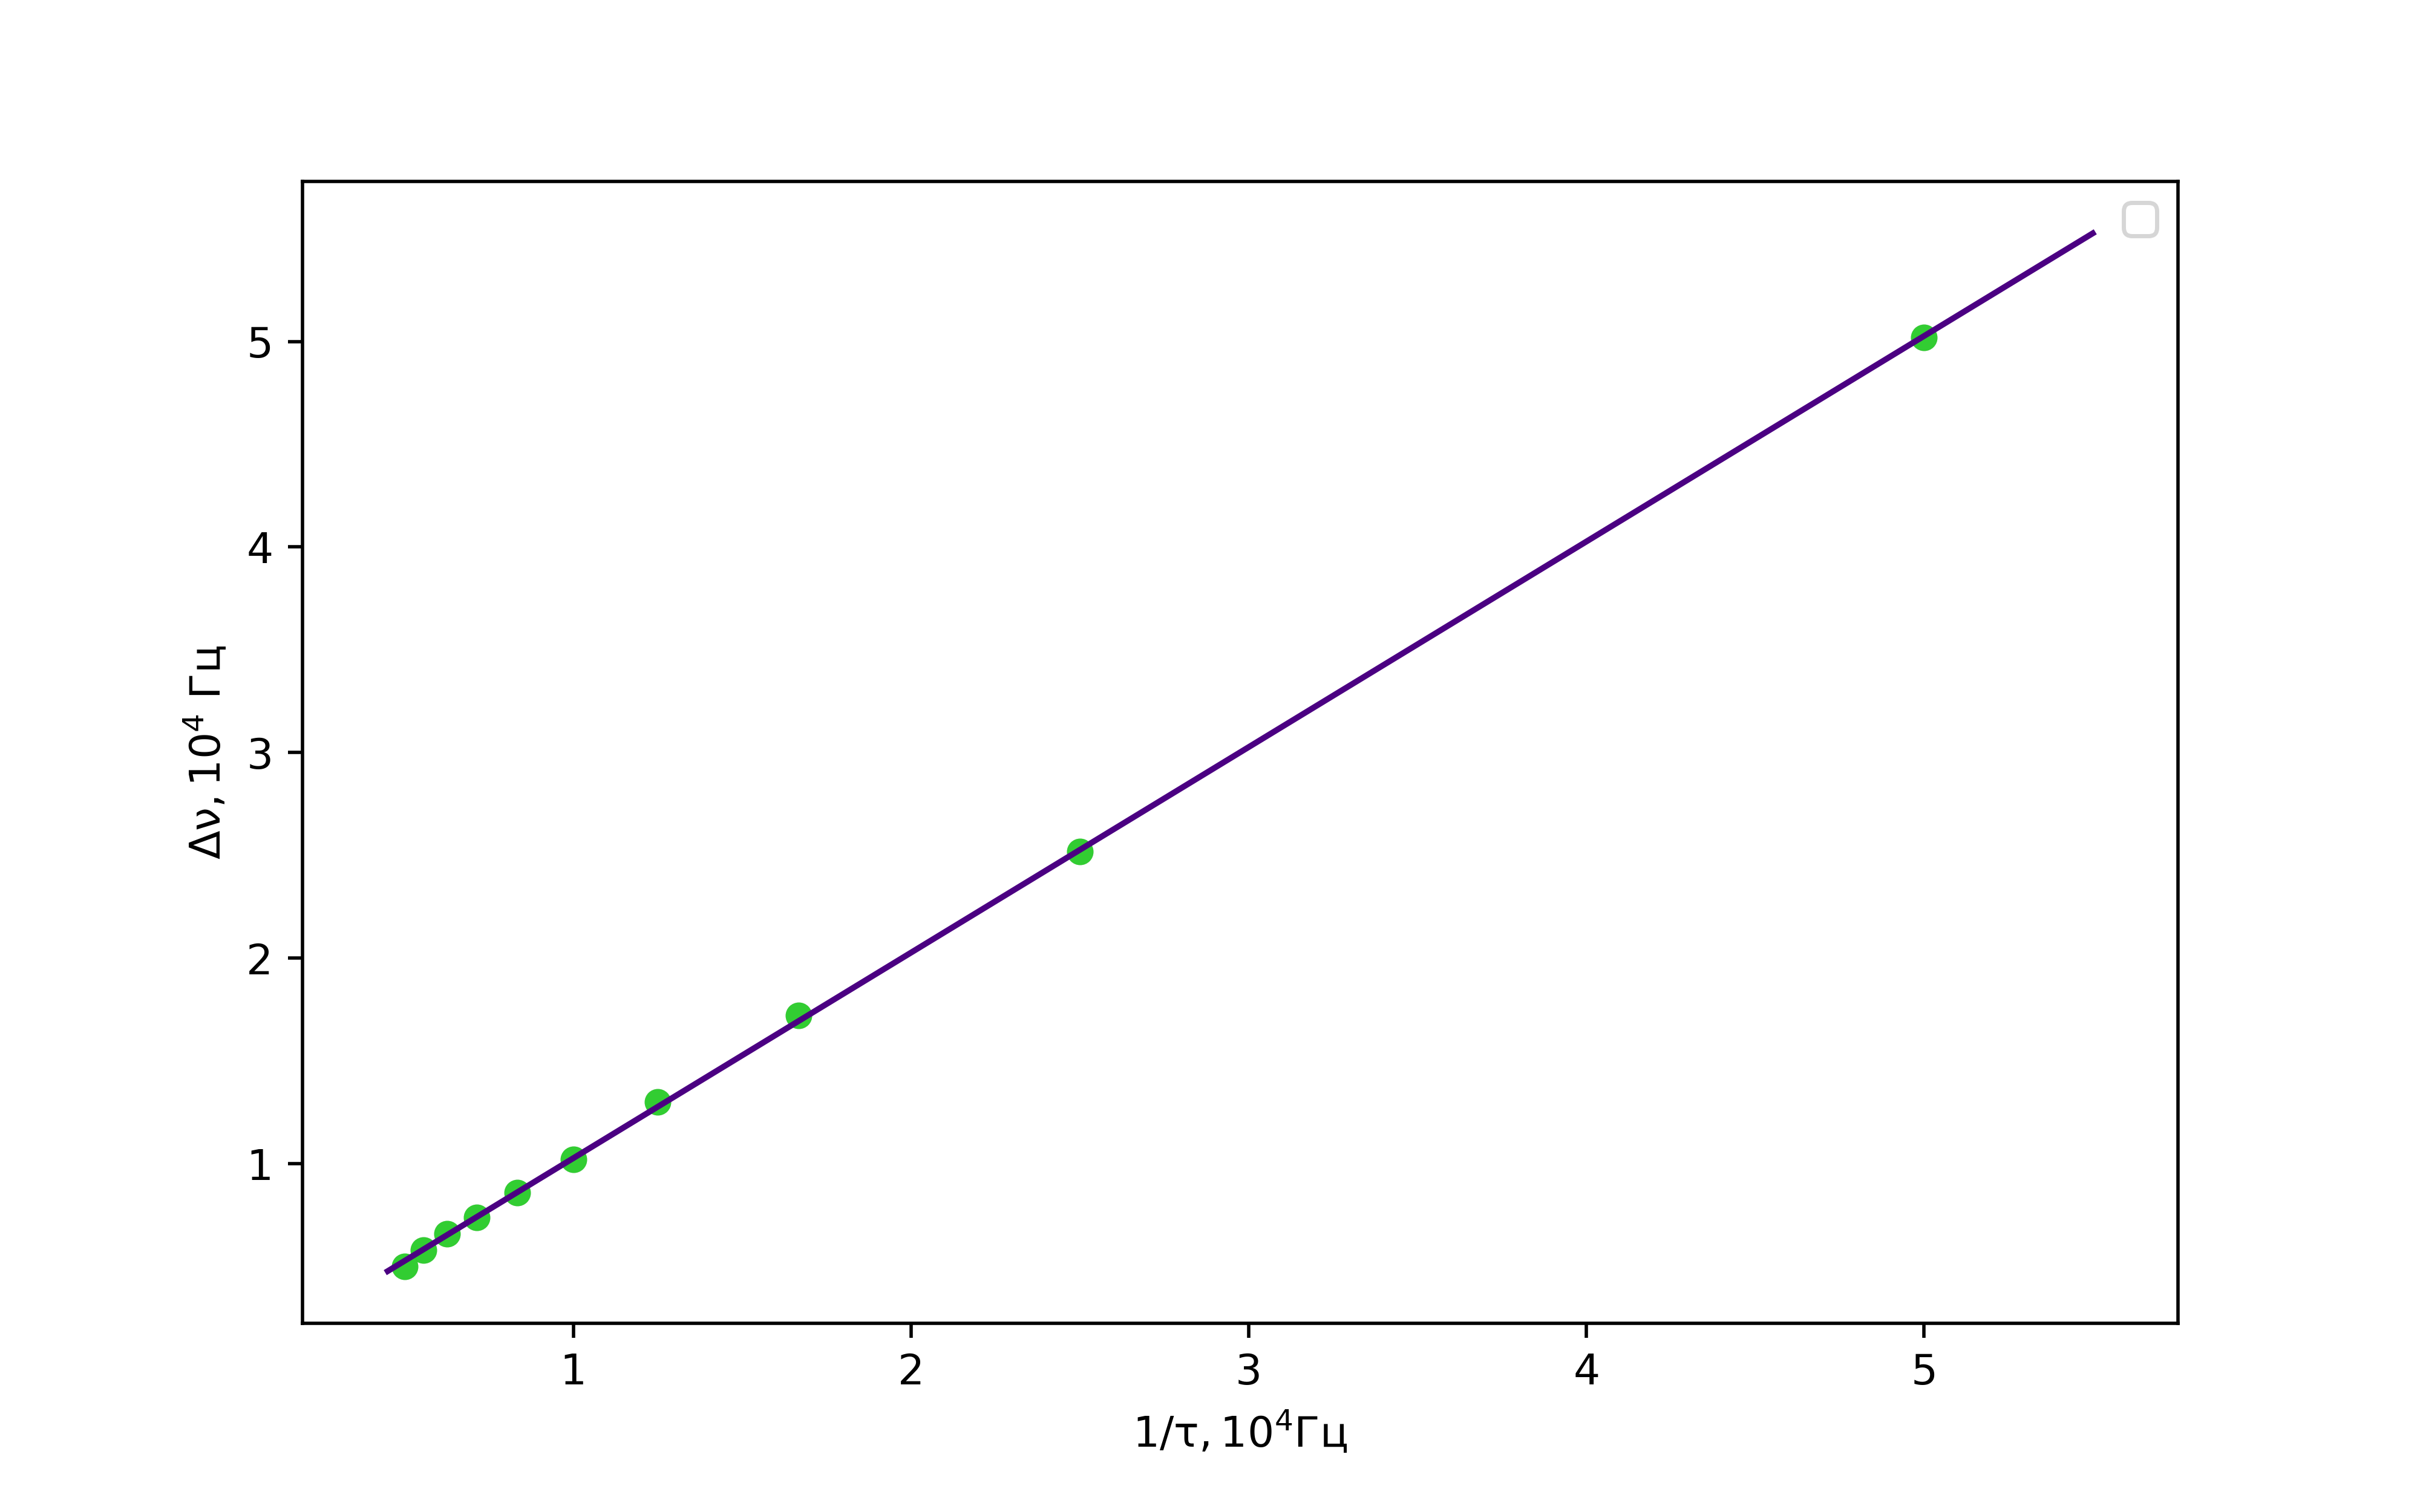
\includegraphics[width=\textwidth]{dnu(tau)}
\caption{Зависимость ширины спектра от длительности спектра для последовательности прямоугольных импульсов} \label{dnu(tau)_img}
\end{center}
\end{figure}
Рассчитан коэффициент наклона прямой:
\begin{equation}
k = 0.9997 \pm 0.0039
\end{equation}
Полученное значение близко к $1$, что подтверждает соотношение неопределенностей. 


Для сравнения экспериментальных и теоретических значений спектра для одного из сигналов (a) рассчитана теоретическую зависимость и изображена на графике \ref{теор}. Теоретический и экспериментальный спектр похожи.

\begin{figure}[h!]
\begin{center}
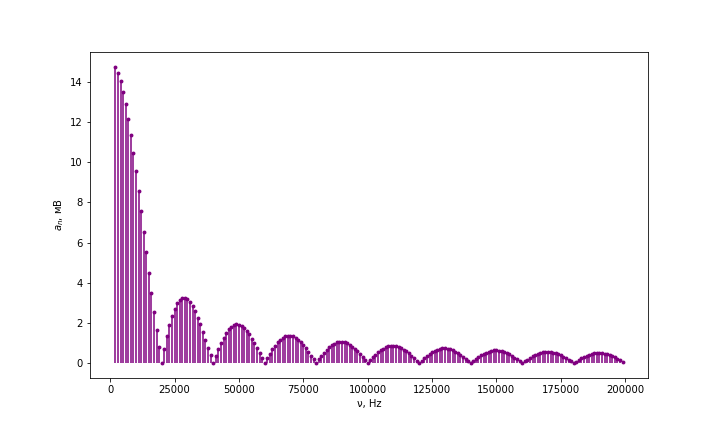
\includegraphics[width=\textwidth]{a(n)}
\caption{Теоретический спектр прямоугольных импульсов из \cite{labnik}} \label{теор}
\end{center}
\end{figure}

\subsection{Исследование спектра периодической последовательности цугов гармонических колебаний}
Для исследования спектра периодической последовательности цугов гармонических колебаний на генераторе создан сигнал последовательности синусоидальных цугов с разными параметрами, по которому на экране осциллографа получен спектр. (рис. \ref{спектр_цуги})

\begin{figure}[h!]
\begin{minipage}[h!]{0.47\linewidth}
\center{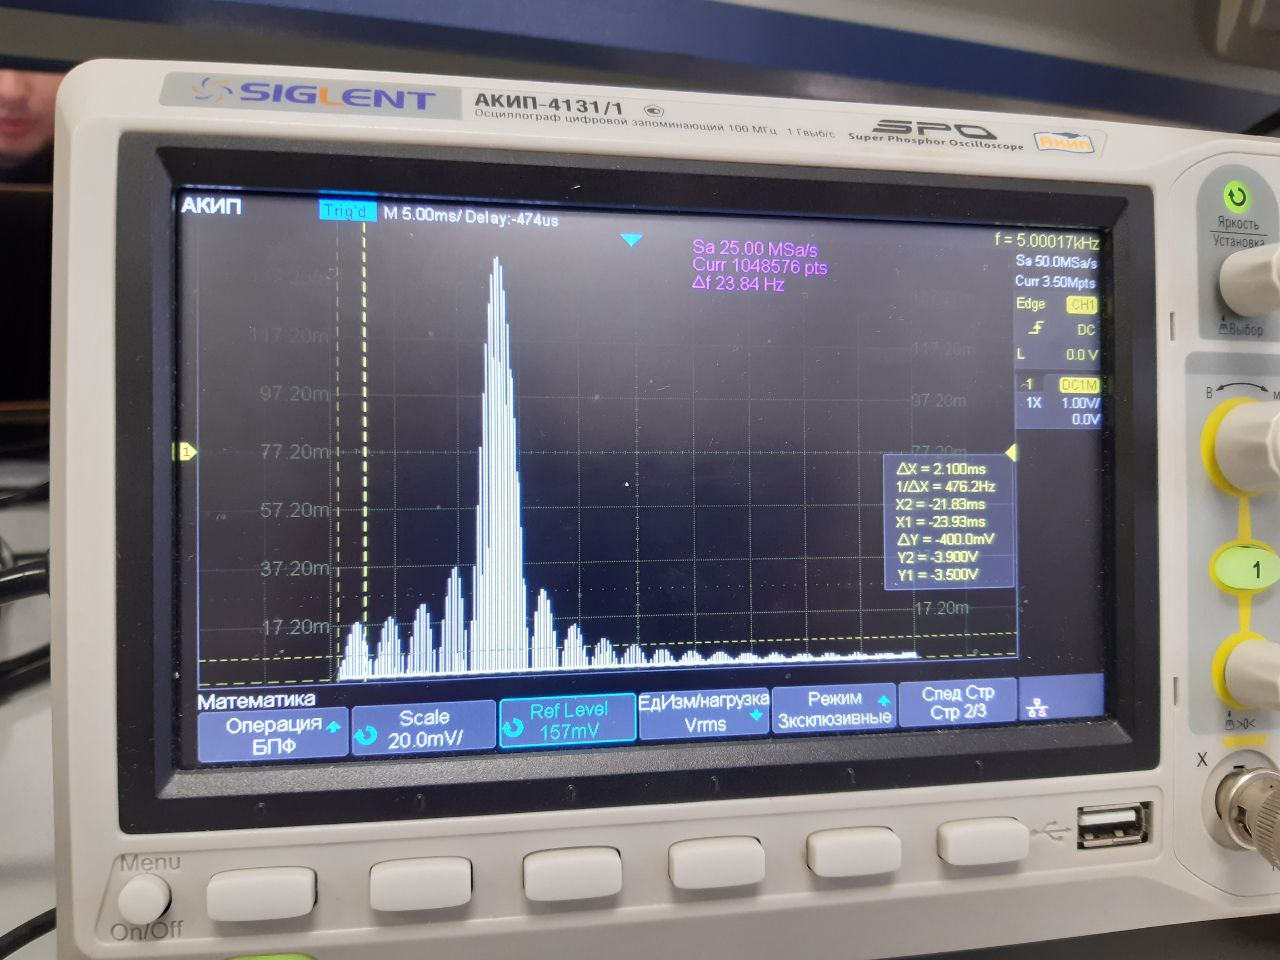
\includegraphics[width=1\linewidth]{2_1}} a) $\nu = 50 кГц, T = 1 мс, N = 5$\\
\end{minipage}
\hfill
\begin{minipage}[h!]{0.47\linewidth}
\center{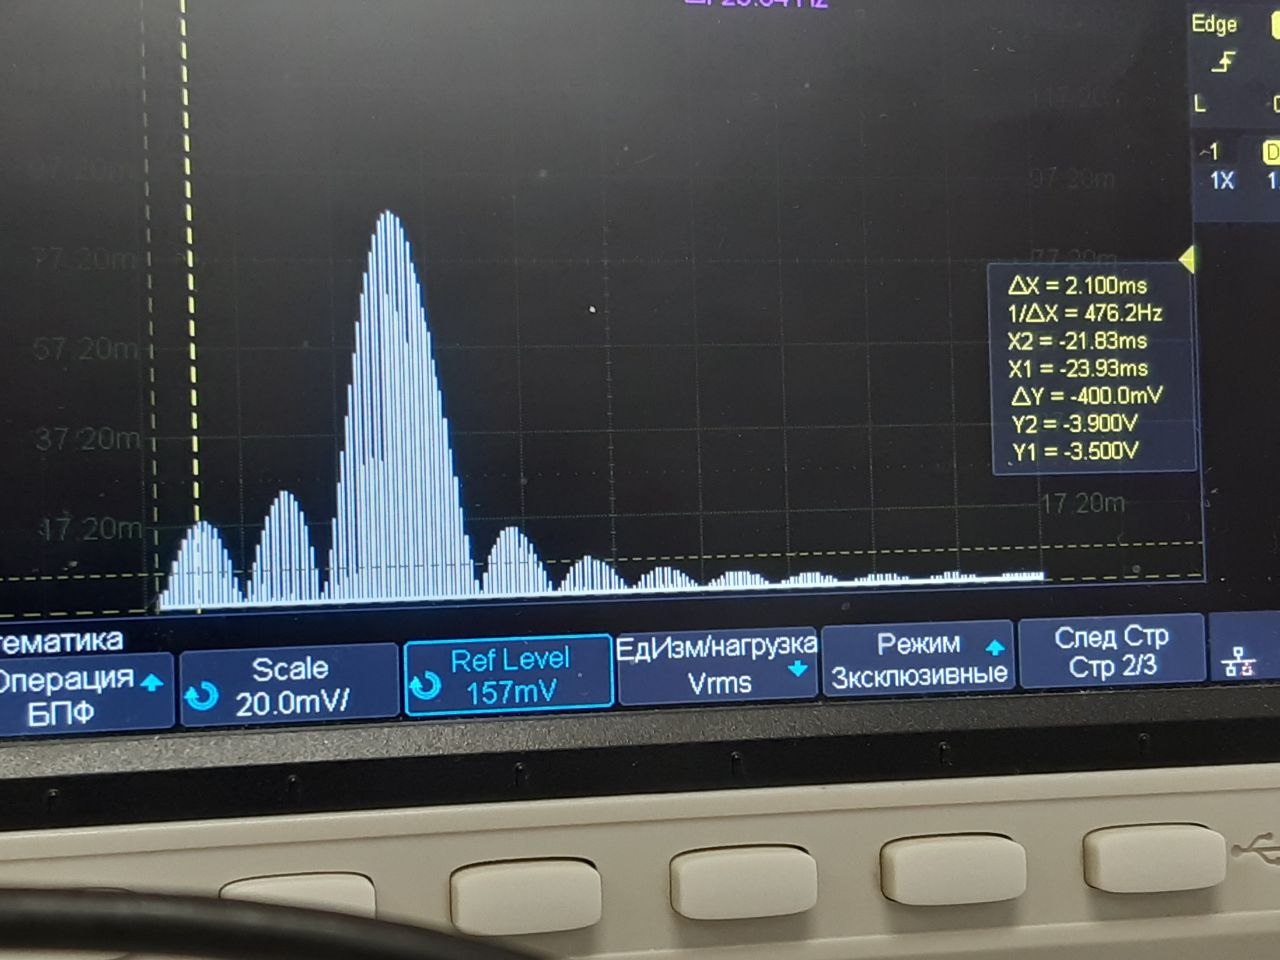
\includegraphics[width=1\linewidth]{2_2}} \\b) $\nu = 50 кГц, T = 1 мс, N = 3$
\end{minipage}
\vfill
\begin{minipage}[h!]{0.47\linewidth}
\center{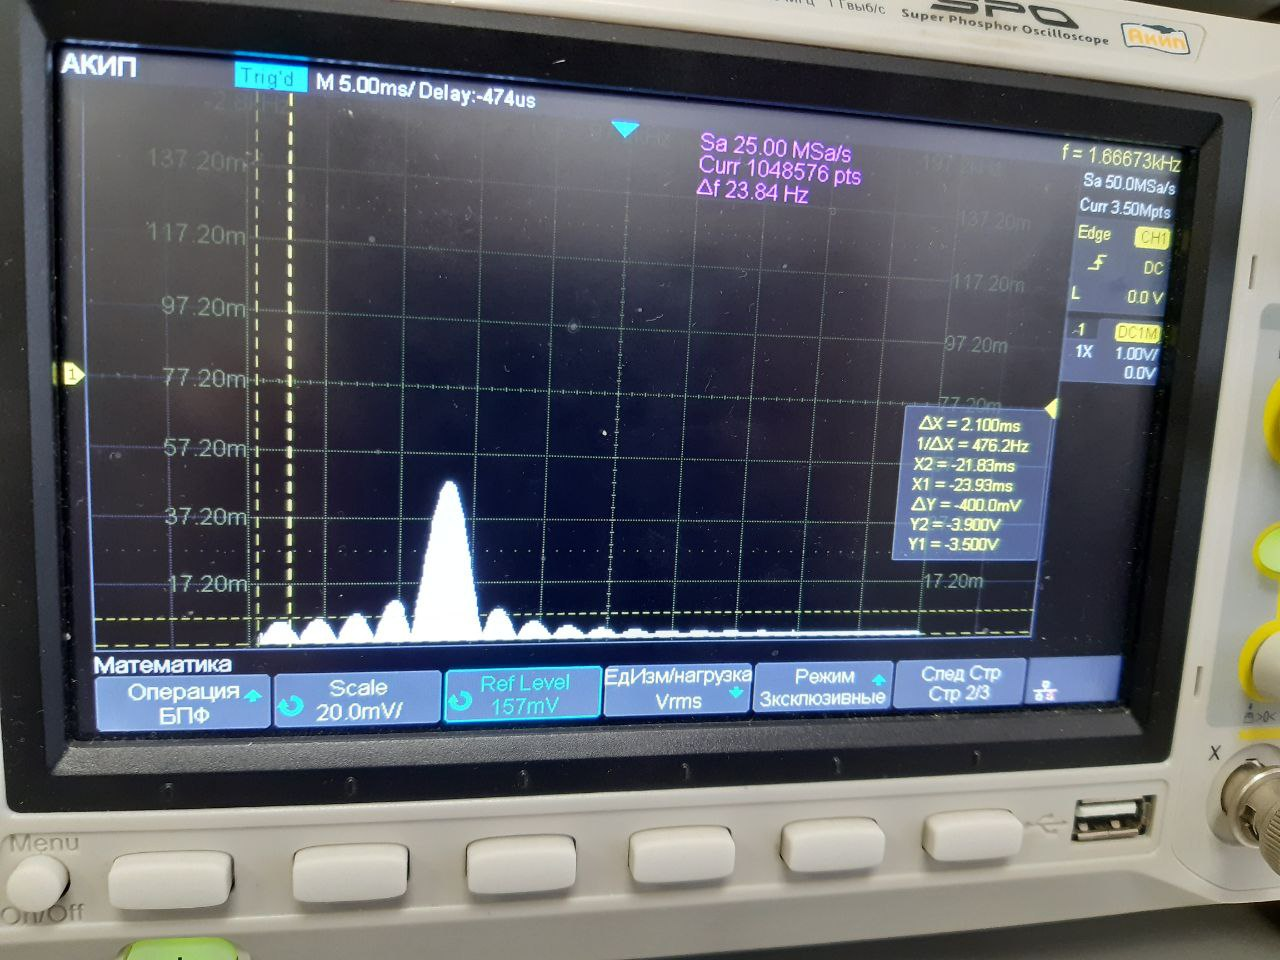
\includegraphics[width=1\linewidth]{2_3}} c) $\nu = 50 кГц, T = 3 мс, N = 5$ \\
\end{minipage}
\hfill
\begin{minipage}[h!]{0.47\linewidth}
\center{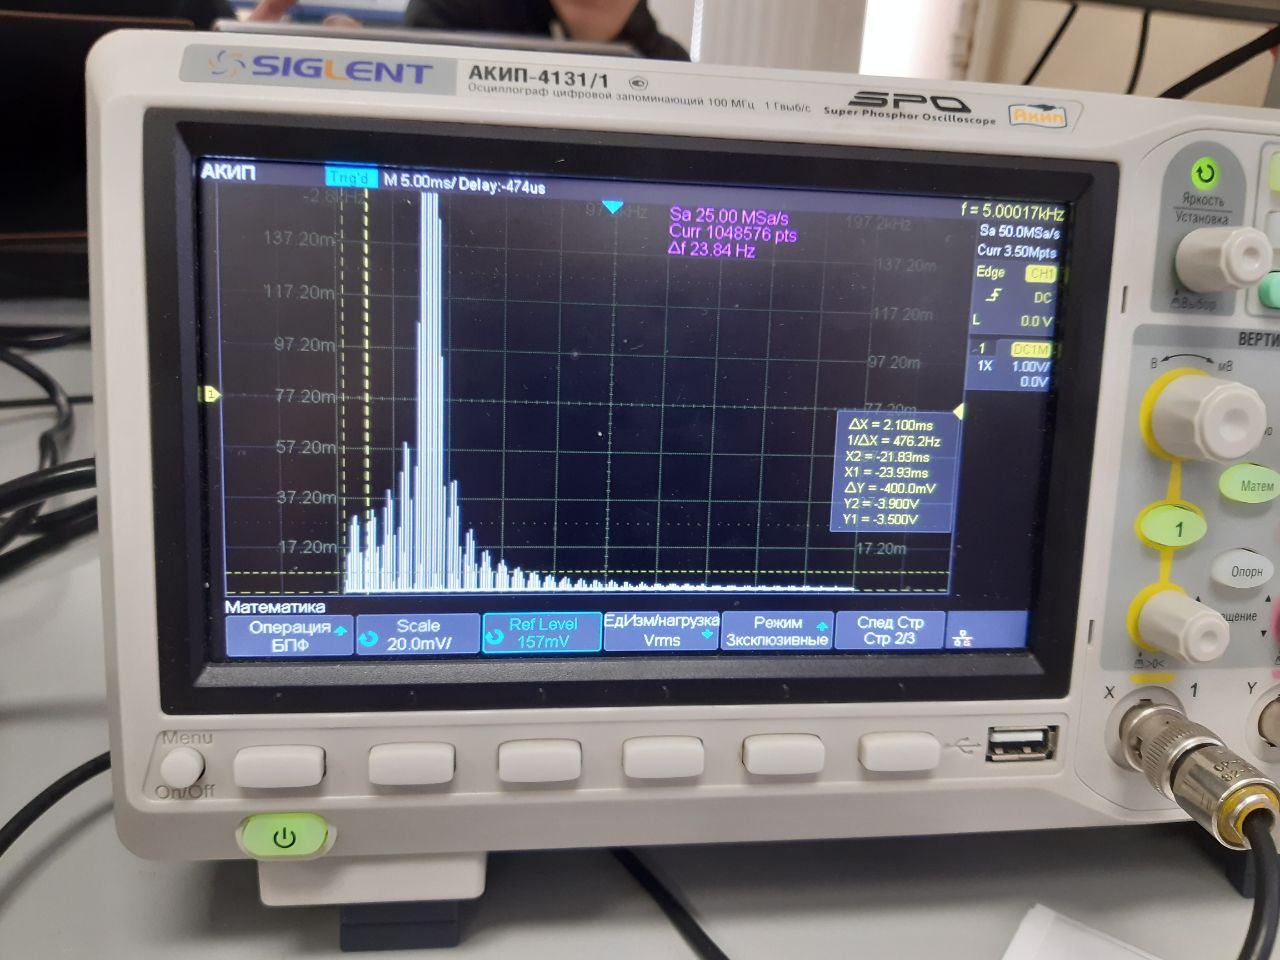
\includegraphics[width=1\linewidth]{2_4}} d) $\nu = 30 кГц, T = 1 мс, N = 5$ \\
\end{minipage}
\vfill
\begin{minipage}[h!]{0.47\linewidth}
\center{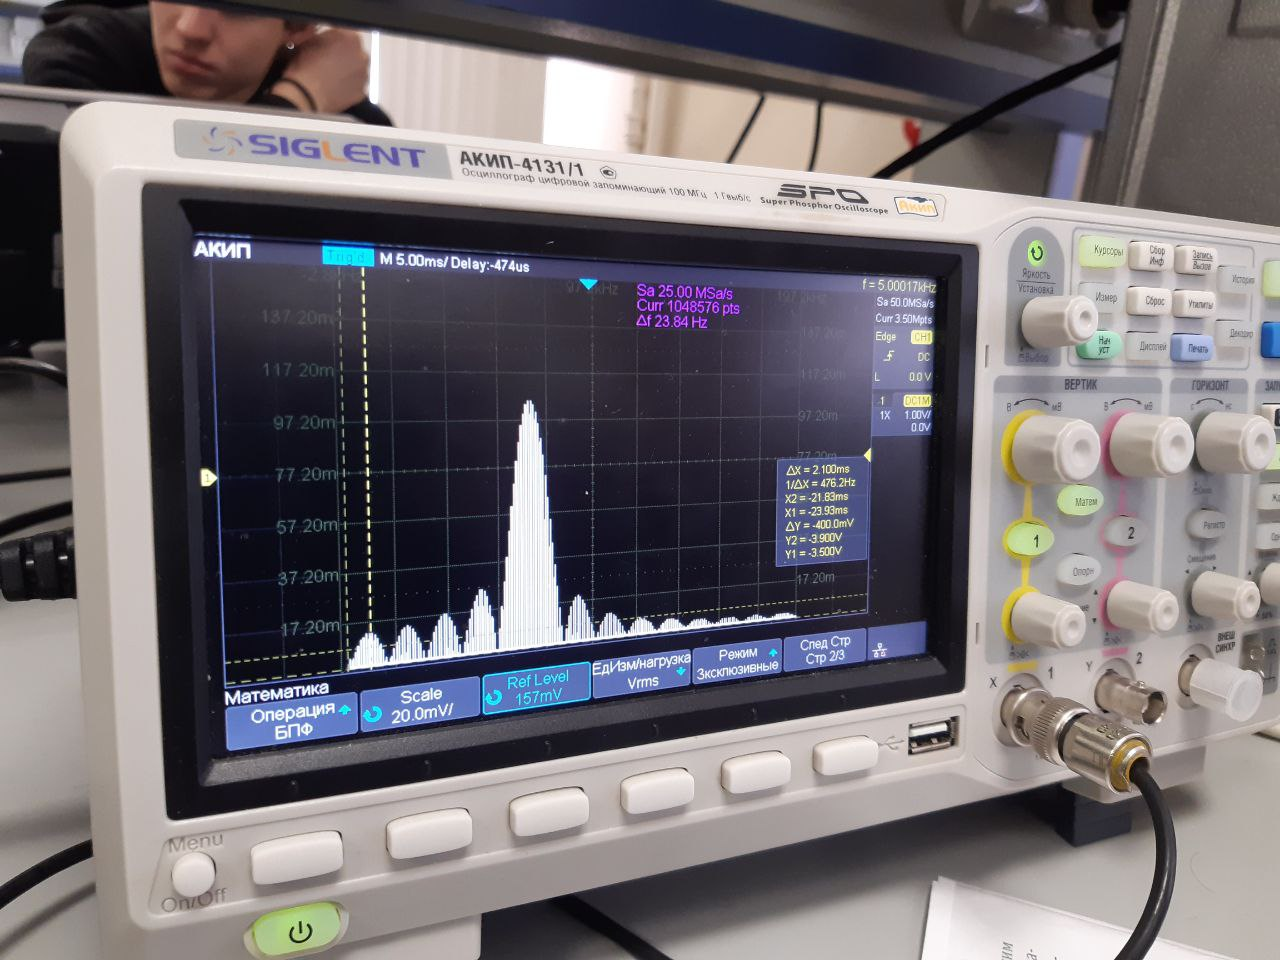
\includegraphics[width=1\linewidth]{2_5}} \\e) $\nu = 70 кГц, T = 1 мс, N = 5$
\end{minipage}
\caption{Вид спектра для периодической последовательности цугов при разных частотах несущей $\nu_0$ = 50 кГц, периодах повторения $T$ = 1 мс, числах
периодов в одном импульсе $N$ = 5}
\label{спектр_цуги}
\end{figure}

Для проверки соотношения неопределенностей для данного сигнала при фиксированной длительности импульсов $\tau$ = 50 мкс измерены расстояния между соседними спектральными компонентами от периода повторения импульсов (табл. \ref{dnu(T)_tbl}, рис. \ref{dnu(T)_img})

\begin{table}[h!]
\caption{Зависимость расстояния между соседними спектральными компонентами от периода повторения импульсов при $\nu_0$ = 50 кГц и $N$ = 5} \label{dnu(T)_tbl}
\begin{tabular}{|l|l|}
\hline
T, ms & $\delta \nu$, Hz \\ \hline
0.2   & 6250    \\ \hline
1     & 2778    \\ \hline
1.5   & 4167    \\ \hline
2     & 1042    \\ \hline
2.5   & 1190    \\ \hline
3     & 735     \\ \hline
3.5   & 893     \\ \hline
4     & 1000    \\ \hline
4.5   & 1042    \\ \hline
5     & 1190    \\ \hline
\end{tabular}
\end{table}

\begin{figure}[h!]
\begin{center}
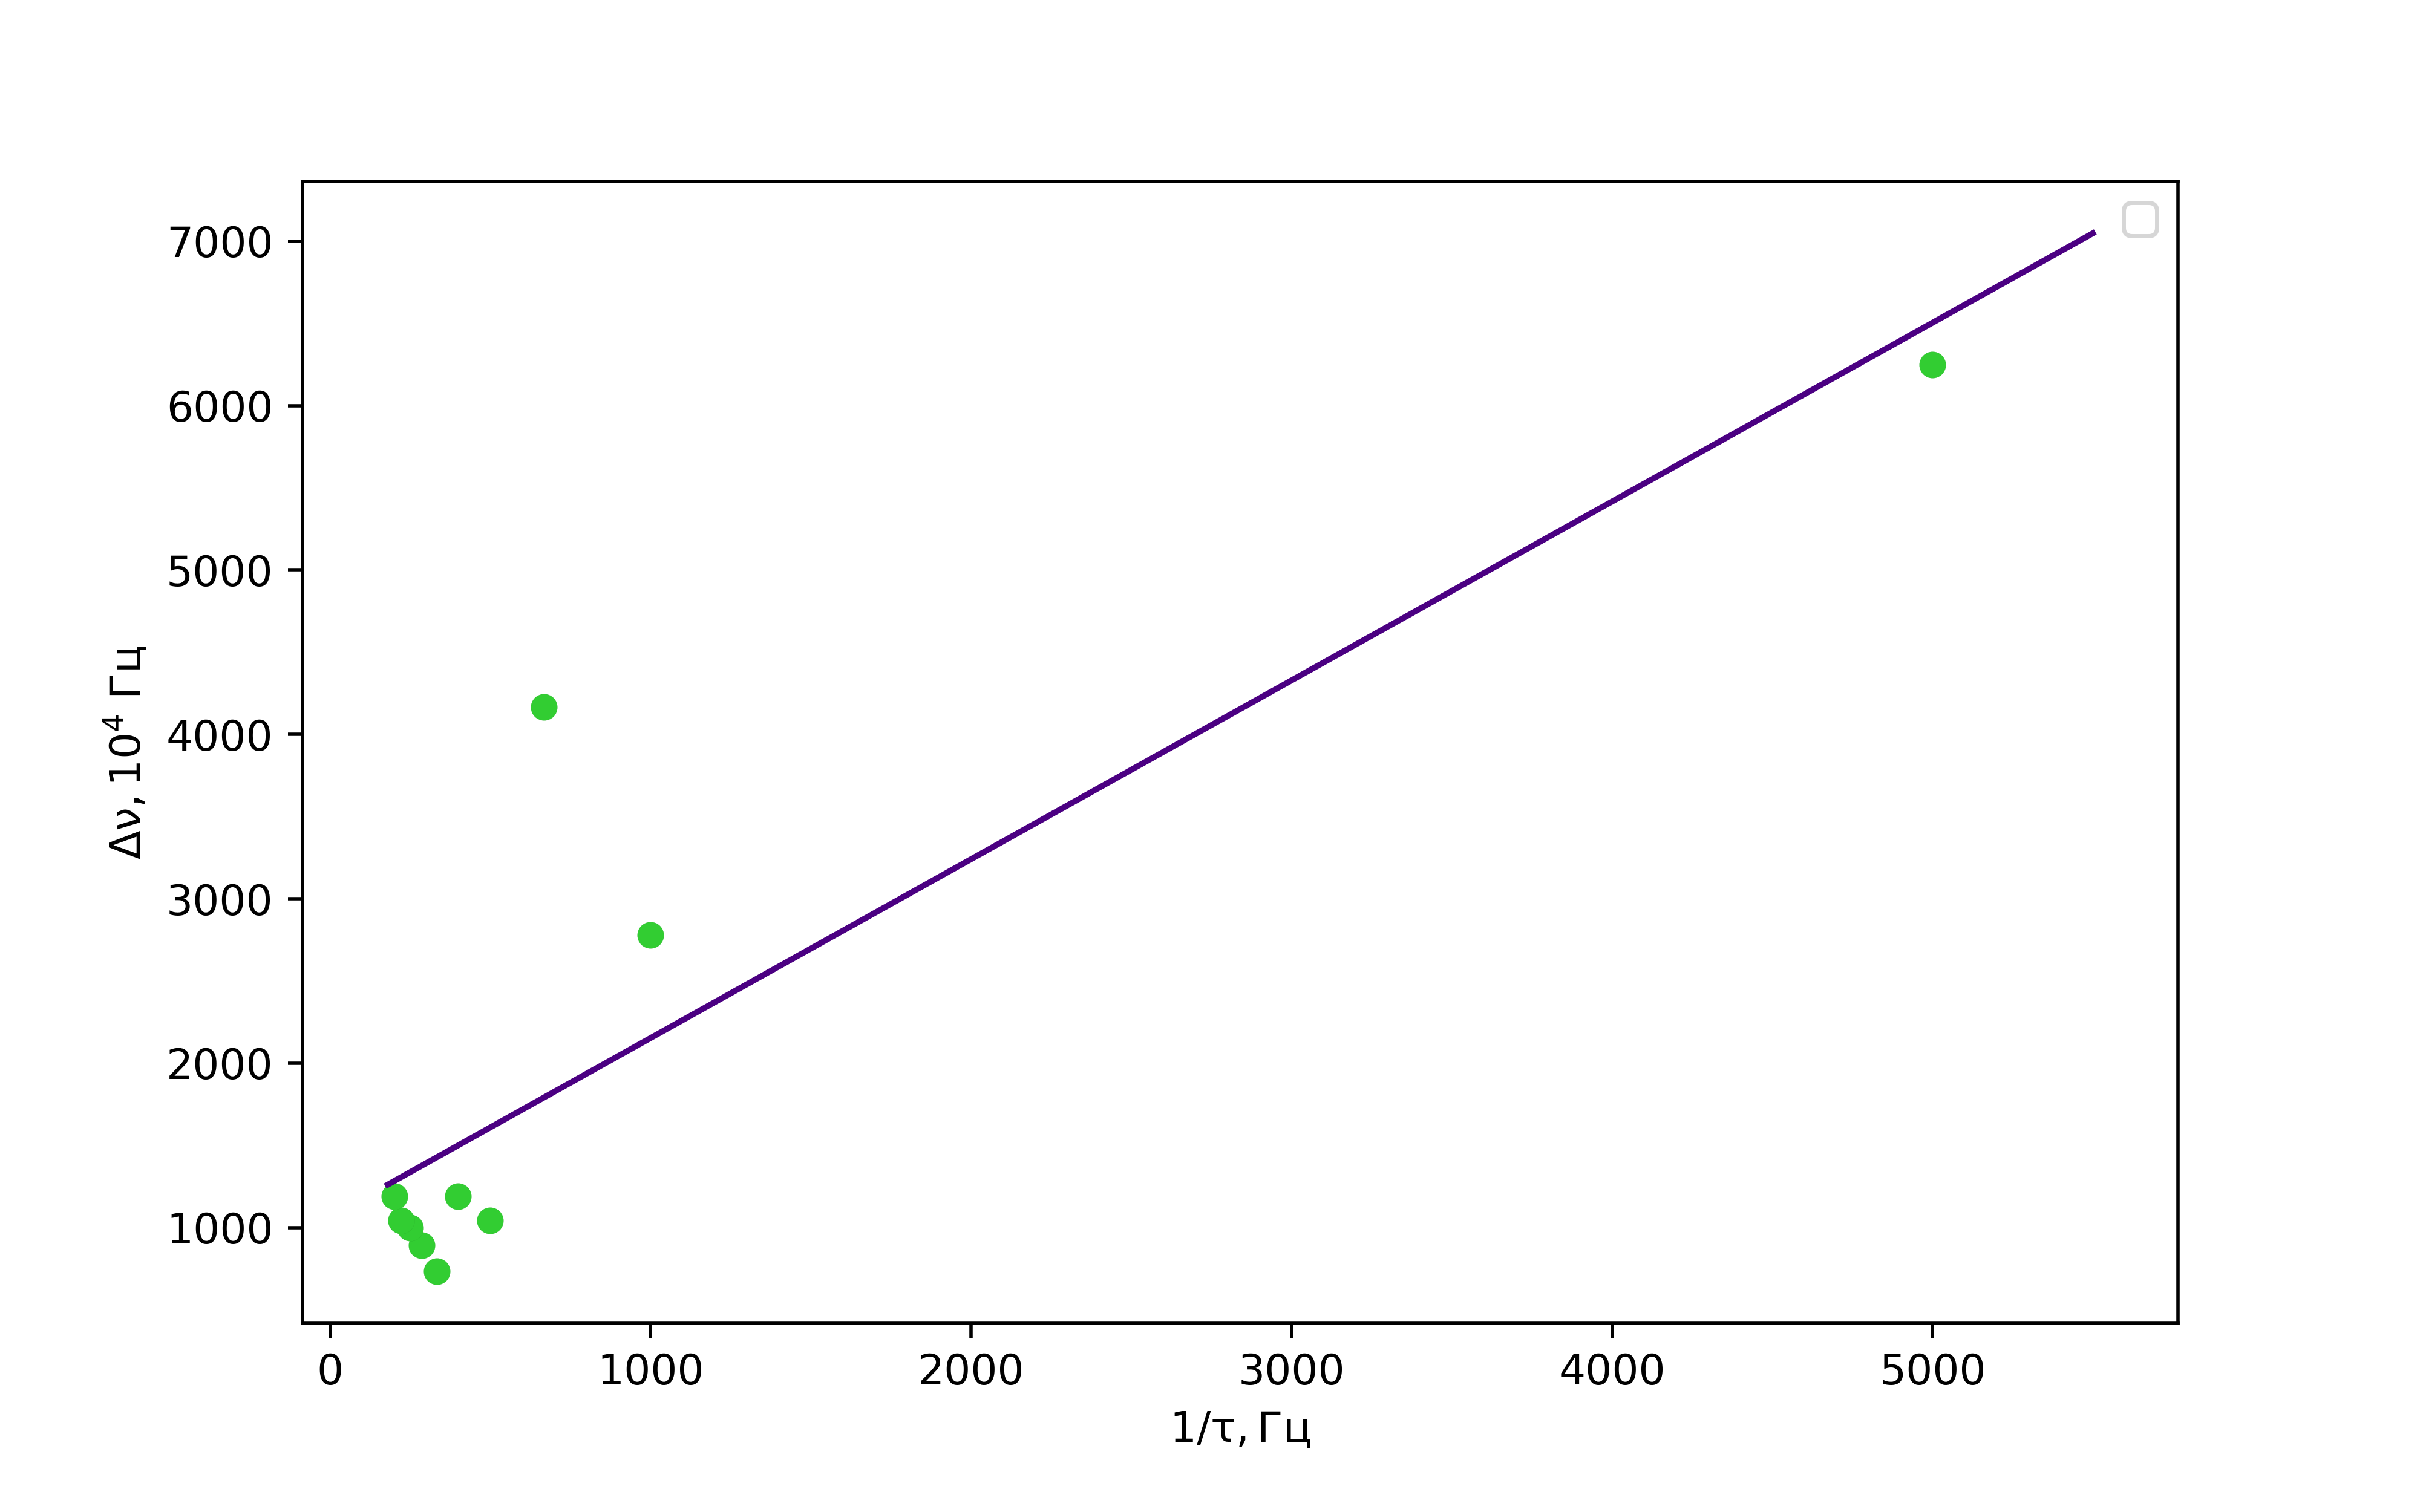
\includegraphics[width=0.9\textwidth]{T(dnu)}
\caption{Зависимость расстояния между соседними спектральными компонентами от периода повторения импульсов} \label{dnu(T)_img}
\end{center}
\end{figure}

Теоретически известно (\cite{labnik}) точки должны хорошо ложиться на прямую, однако из графика видно, что это не так. Проблема заключается в снятии данных (был выбран неверный канал при курсорных измерениях). Поэтому подтвердить справедливость соотношения неопределенности невозможно. 

\subsection{Исследование спектра гармонических сигналов, модулированных по амплитуде}
Для исследования спектра гармонических сигналов, модулированных по амплитуде на генераторе создан сигнал, модулированный по амплитуде, по которому на экране осциллографа получается спектр (\ref{мод}).
\begin{figure}[h!]
\begin{center}
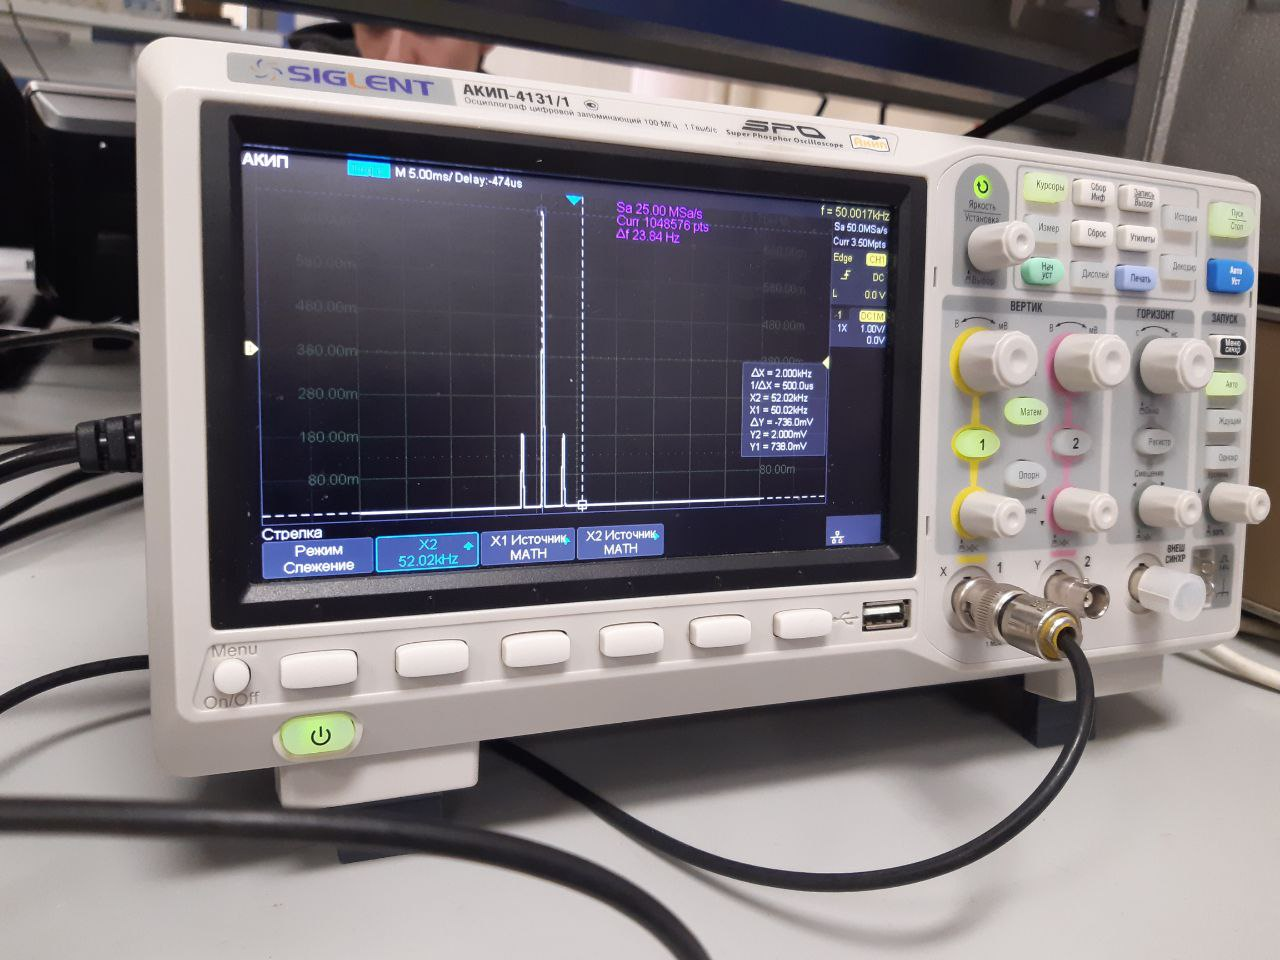
\includegraphics[width=\textwidth]{3}
\caption{Спектр сигнала, модулированного по амплитуде, при частоте несущей $\nu_0$ = 50 кГц, частоте модуляции $\nu_{мод}$ = 2 кГц} \label{мод}
\end{center}
\end{figure}
Измерена с помощью осциллографа глубину модуляции:
\begin{equation}
m = \dfrac{A_{max}-A_{min}}{A_{max}+A_{min}} = \dfrac{1.54 - 0.04}{1.54 + 0.04} = 0.5, что сходится с установленным на генераторе
\end{equation}
Для проверки теоретической зависимости, изменяя глубину модуляции, измерена $\dfrac{a_{бок}}{а_{осн}}$ (табл. \ref{mod_tbl} и рис. \ref{mod_img}).

\begin{table}[h!]
\caption{Зависимость $\dfrac{a_{бок}}{а_{осн}}$ от $m$ при частоте несущей $\nu_0$ = 50 кГц, частоте модуляции $\nu_{мод}$ = 2 кГц}
\label{mod_tbl}
\begin{tabular}{|l|l|l|}
\hline
m   & a\_бок & a\_центр \\ \hline
50  & 186    & 738      \\ \hline
10  & 38     & 738      \\ \hline
20  & 74     & 738      \\ \hline
30  & 110    & 738      \\ \hline
40  & 150    & 738      \\ \hline
60  & 222    & 738      \\ \hline
70  & 258    & 738      \\ \hline
80  & 298    & 738      \\ \hline
90  & 334    & 738      \\ \hline
100 & 370    & 738      \\ \hline
\end{tabular}
\end{table}
\begin{figure}[h!]
\begin{center}
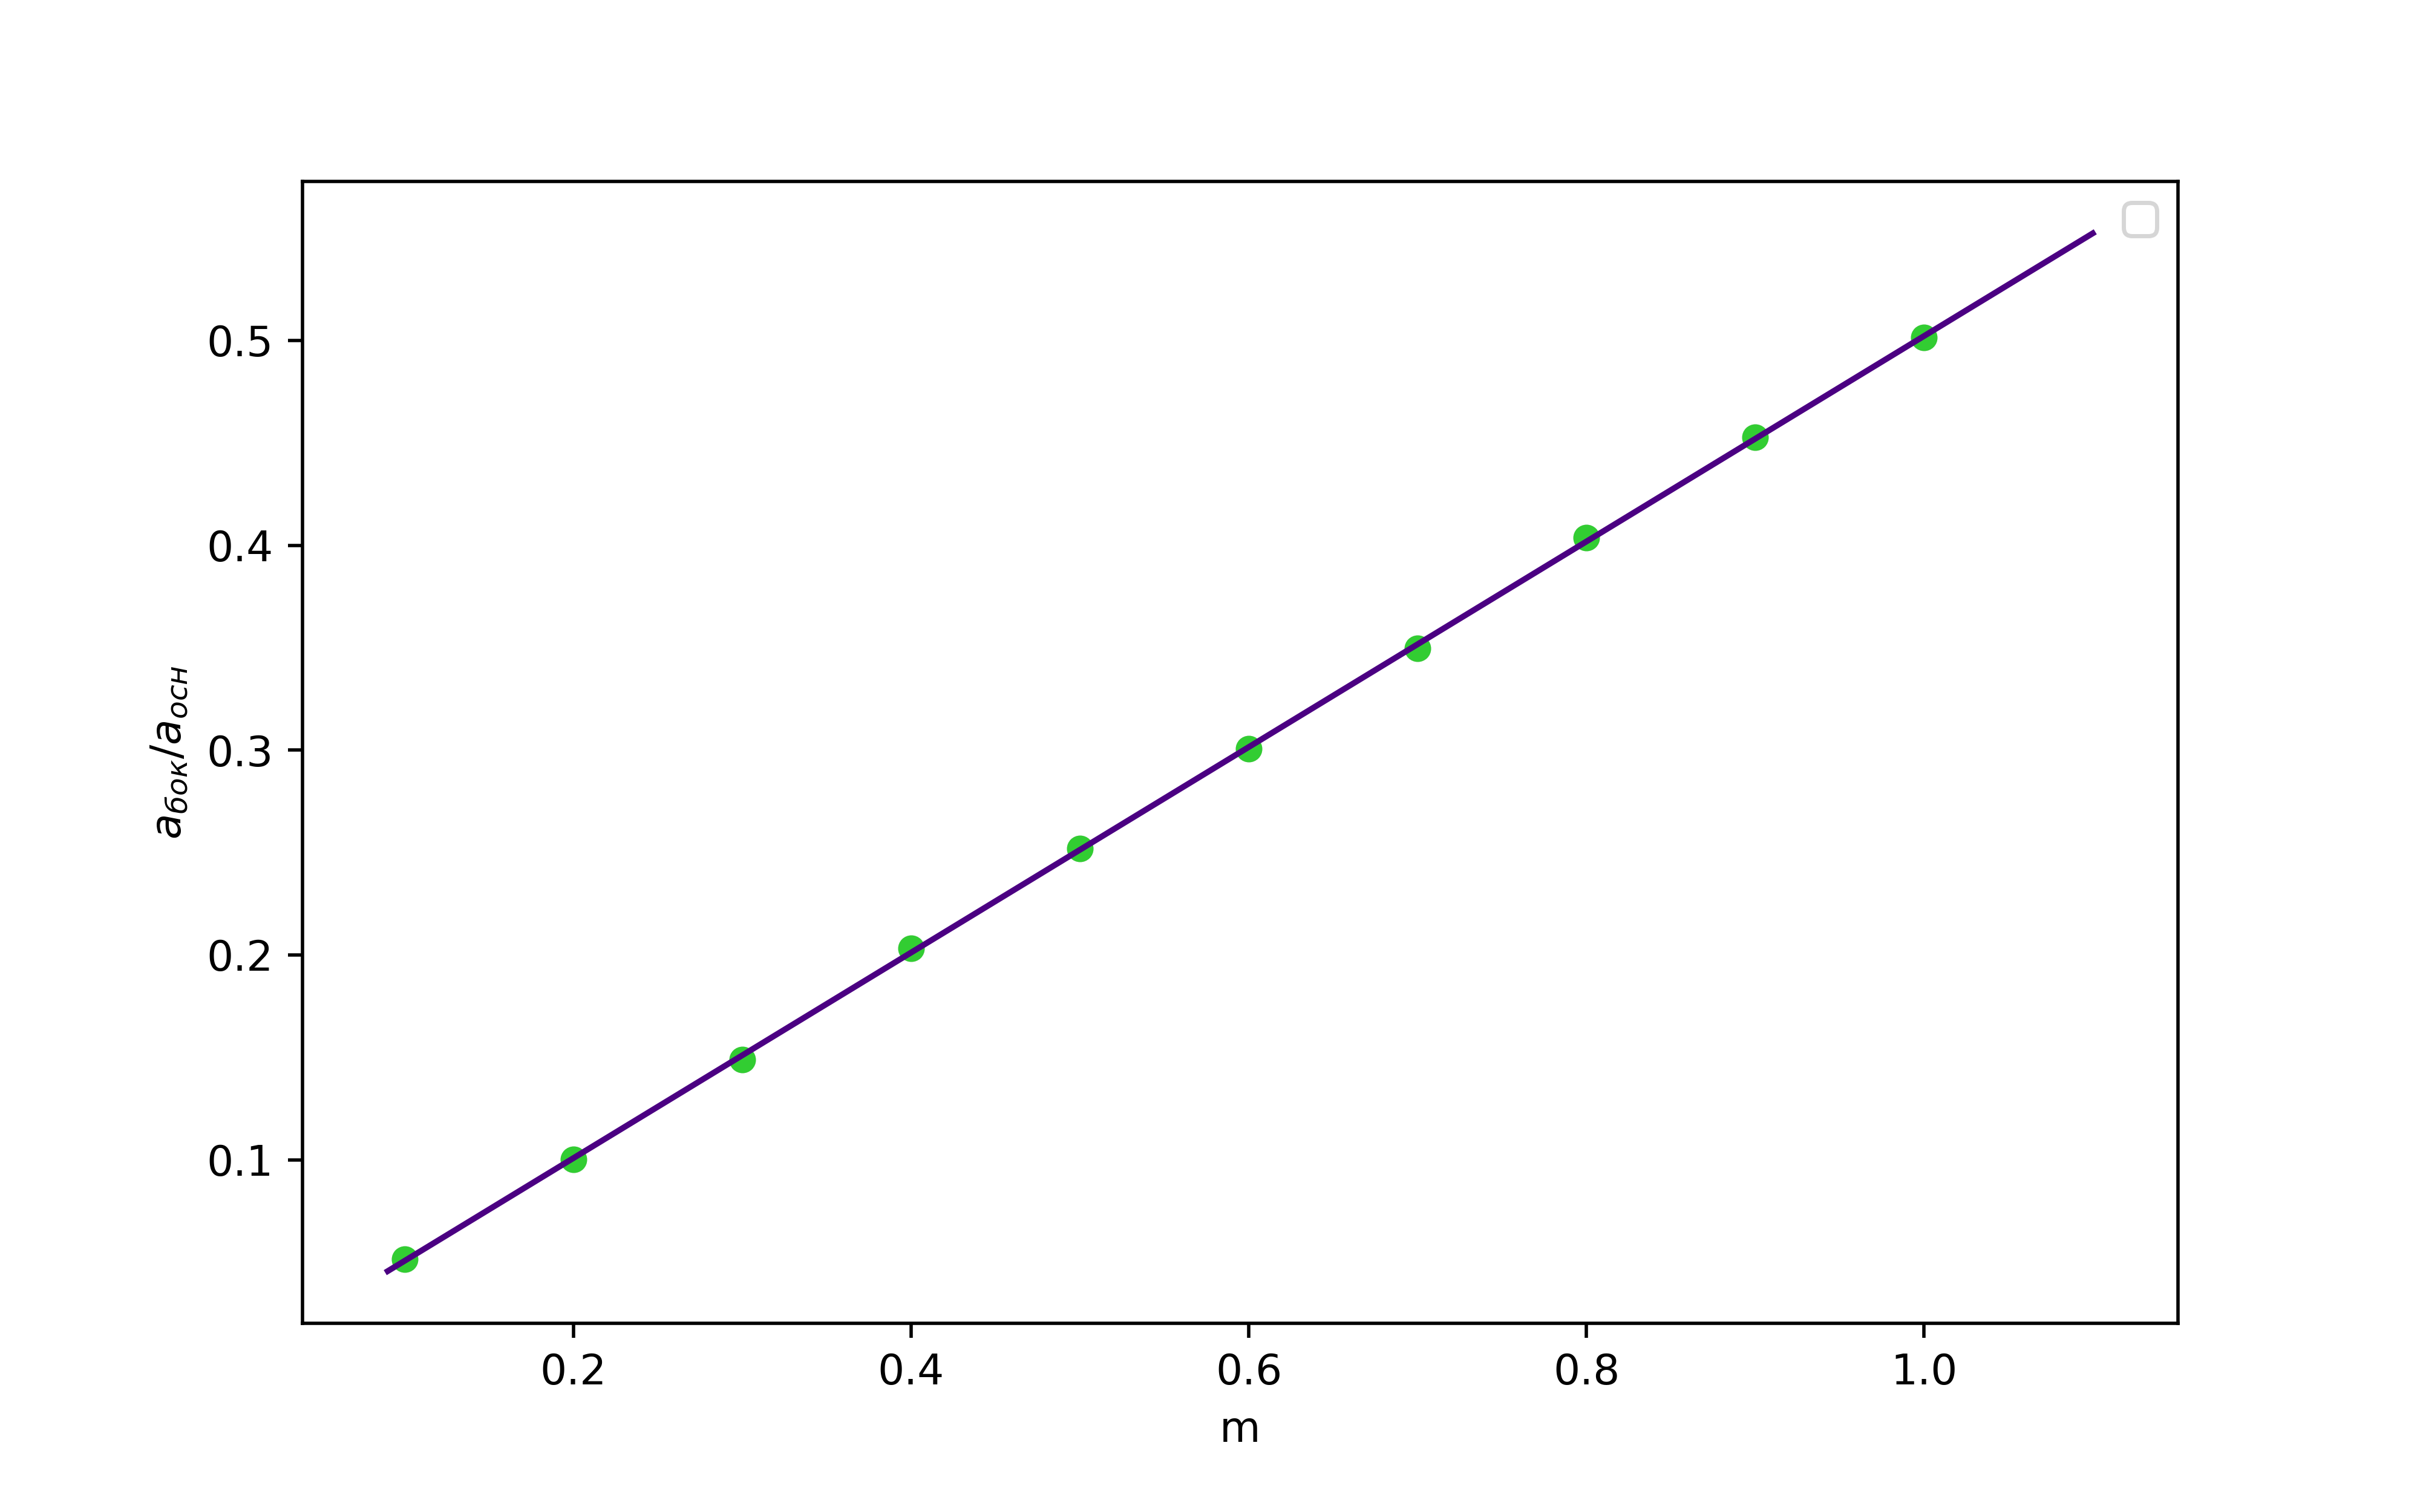
\includegraphics[width=0.9\textwidth]{a(m)}
\caption{Зависимость $\dfrac{a_{бок}}{а_{осн}}$ от $m$ при частоте несущей $\nu_0$ = 50 кГц, частоте модуляции $\nu_{мод}$ = 2 кГц} \label{mod_img}
\end{center}
\end{figure}
Определен коэффициент наклона прямой:
\begin{equation}
k = 0.502 \pm 0.002
\end{equation} 
Результат сходится с предсказанным теоретически (0.5).

\section{Выводы}


1. При исследовании последовательности прямоугольных импульсов получена зависимость ширины спектра от длительности импульса, что подтверждает соотношение неопределенностей для данного вида сигнала: $\tau \cdot \Delta\nu \sim 1$.

2. Проверены теоретические расчеты спектра при прямоугольных импульсах (теоретическая и экспериментальная картины схожи).

3. При обработке данных от спектра периодической последовательности цугов была обнаружена ошибка при снятии данных, что не позволило проверить соотношение неопределенностей.

4. Получен угол наклона графика зависимости $\dfrac{a_{бок}}{а_{осн}}$ от $m$ (0.5), подтверждено теоретическое значение этого угла (0.5).


\begin{thebibliography}{}
    \bibitem{labnik}  Никулин М.Г., Попов П.В., Нозик А.А. и др. Лабораторный практикум по общей физике : учеб. пособие. В трех томах. Т. 2. Электричество и магнетизм
\end{thebibliography}


\end{document}